\chapter{Preparation of the data}

Before any analysis of the acquired data could begin, it was necessary to load and extract the content of the xvi files produced by the thermal camera.  

\section{Dividing the data into frames}

Data acquired from the thermal camera using the Xeneth 2.6 software is saved as an xvi file\fxnote{what is xvi}. These files was loaded and read into Matlab R2017b as an uint16 vector file. Before the frames could be separated from the xvi file, the header in front of the files needed to be excluded. The header contained 307729 data points. With the header removed, the frame separation could be carried out. This was done by first calculating the size of one frame. When knowing that each frame would have the dimensions of 640x480 pixels, the size of one frame would correspond to 307200 data points for each frame. It should be noticed that each frame also contained a 16 bit header, so this should be added to the size of each frame. The number of frames was calculated by dividing the length of one frame by the entire length of the data file containing all frames, without the file header. By this calculation it was known how many frames the file contained. The data points for each frame were trimmed for its specific frame header and reshaped from a vector into a matrix and verified by showing the images. 
The images contain the pixel intensities of values from 0 to 65535, which is corespondent to the size of the uint16 bit file. 
% or if it is the int16 bit file it's values from -32768 to 32767. But the uint16 image looks better and is easier to see, so i think we should use thatone - it won't affect the dataanalysis. 

% Maybe write about temperature convertion

\begin{figure}[H]
	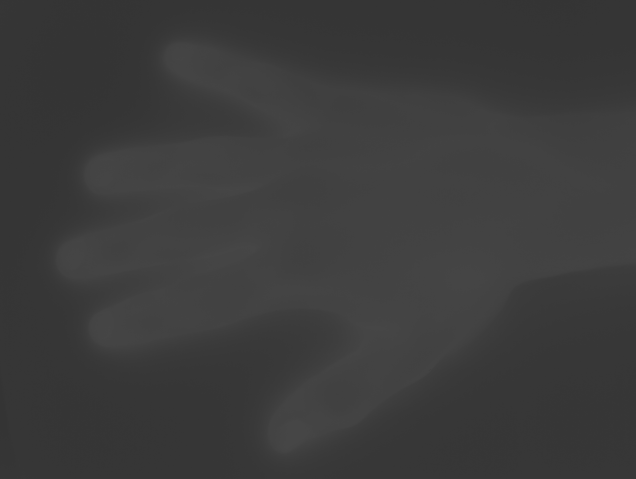
\includegraphics[width=0.6\textwidth]{figures/uint16Hand}  %<--but is not needed.
	\caption{Image of one frame from subject one after separation.}
	\label{fig:hand}  %<--give the figure a label, so you can reference!
\end{figure}